% 110-27(인쇄 110쪽) — 개념 33 27번 오른쪽의 빈 표준정규분포곡선(학생이 확률을 색칠할 자리).
% 스캔 화질이 낮아 TikZ 로 다시 그림. 라벨은 원문에 있는 것만($0$, $z$)이고 색칠은 하지 않는다(답이 그림에서 읽히지 않게).
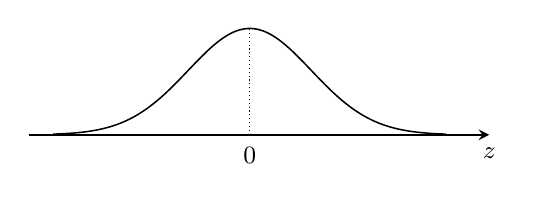
\begin{tikzpicture}[x=0.78cm, y=1.35cm, line width=0.55pt, font=\small]
  \draw[->, >=stealth, line width=0.7pt] (-3.6,0) -- (3.9,0) node[below=1pt] {$z$};
  \draw plot[domain=-3.2:3.2, samples=110, smooth] ({\x},{exp(-\x*\x/2)});
  \draw[densely dotted, line width=0.4pt] (0,0) -- (0,1);
  \node[below=1pt] at (0,0) {$0$};
\end{tikzpicture}
